\documentclass[a4paper,fleqn]{cas-sc}   %{article}
%remove ORCID footnote
\renewcommand{\printorcid}{}


%\usepackage{natbib}
\usepackage{float}
\usepackage{array}
\usepackage{multirow}
\usepackage{booktabs}
\usepackage{adjustbox}
\usepackage[style=authoryear-icomp,
uniquelist=false,
maxnames=2,
minnames=1,
maxbibnames=99,
    backend=biber, giveninits=true,
    ibidtracker=false,
    uniquename=false,
    natbib=true]{biblatex}

\addbibresource{DCE_lit_review.bib}
\addbibresource{Used EV.bib}
\addbibresource{EV battery.bib}
\addbibresource{used_EV_lit_review}
% \DeclareNameAlias{default}{family-given}

\usepackage{amsmath}
\usepackage{amssymb}
\usepackage{bm}
\usepackage{hyperref}
\usepackage{graphicx}

% Force floats to appear where inserted, not deferred to end of document.
% Use [H] specifier on every \begin{figure} and \begin{table}.
% The parameters below allow LaTeX to place floats very liberally.
\renewcommand{\topfraction}{0.99}
\renewcommand{\bottomfraction}{0.99}
\renewcommand{\textfraction}{0.01}
\renewcommand{\floatpagefraction}{0.99}
\setcounter{topnumber}{20}
\setcounter{bottomnumber}{20}
\setcounter{totalnumber}{40}

% add line number
\usepackage{lineno}
\pagewiselinenumbers

%\usepackage{titlesec}
%\titlespacing*{\section}{0pt}{6pt}{3pt}  
%\titlespacing*{\subsection}{0pt}{6pt}{3pt} 
%\titlespacing*{\subsubsection}{0pt}{6pt}{3pt}

% remove the "preprint"
\ExplSyntaxOn \cs_gset:Npn \__first_footerline: { \group_begin: \small \sffamily \__short_authors: \group_end: } \ExplSyntaxOff

\shortauthors{}

%%%Author macros
\def\tsc#1{\csdef{#1}{\textsc{\lowercase{#1}}\xspace}}
\tsc{WGM}
\tsc{QE}
\tsc{EP}
\tsc{PMS}
\tsc{BEC}
\tsc{DE}
%%%


\begin{document}
\let\WriteBookmarks\relax
\def\floatpagepagefraction{1}
\def\textpagefraction{.001}
\shorttitle{}
%\shortauthors{X. Iogansen et~al.}

%\begin{frontmatter}

\title [mode = title]{Measuring User preferences for Used EVs}                      


\author[1]{Zain {hoda}}
\fnmark[1]
\credit{Conceptualization, Data curation, Methodology, Software, Formal analysis, Writing - Original Draft, Writing - Review \& Editing}

\author[1,2]{Xiatian {Iogansen}}
\fnmark[2]
\credit{Conceptualization, Data curation, Methodology, Writing - Review \& Editing}

\author[2]{Christina {Gore}}
\credit{Conceptualization, Data curation, Methodology, Investigation, Writing - Original draft preparation, Writing - Review \& Editing, Supervision, Project administration, Funding acquisition}
\fnmark[3]
\cormark[1]
\cortext[cor1]{Corresponding author}

\author[2]{Joshua D. {Kneifel}}
\credit{Conceptualization, Data curation, Methodology, Investigation, Writing - Review \& Editing, Supervision, Project administration, Funding acquisition}
\fnmark[4]

\author[1,2]{Sindhu {Ranganath}}
\credit{Data curation, Writing - Original Draft, Writing - Review \& Editing}
\fnmark[5]

\author[1]{John {Helveston}}
\credit{Conceptualization, Methodology, Writing - Review \& Editing, Supervision}
\fnmark[6]


                
\affiliation[1]{organization={Department of Engineering Management and Systems Engineering, George Washington University},
                city={Washington D.C.},
                country={USA}}

\affiliation[2]{organization={Applied Economics Office, Engineering Laboratory, National Institute of Standards and Technology},
                country={USA}}     
                


\fntext[fn1]{zain.hoda@gwu.edu}
\fntext[fn2]{xiatian.iogansen@gwu.edu \& xiatian.iogansen@nist.gov, https://orcid.org/0000-0002-4851-1323}
\fntext[fn3]{christina.gore@nist.gov, https://orcid.org/0000-0002-3586-6918}
\fntext[fn4]{joshua.kneifel@nist.gov}
\fntext[fn5]{sindhu.ranganath@nist.gov, https://orcid.org/0000-0001-5764-9773}
\fntext[fn6]{jph@gwu.edu, https://orcid.org/0000-0002-2657-9191}


\begin{abstract}
This study employs a discrete choice experiment (DCE) to measure consumer willingness to pay (WTP) for powertrain type and vehicle attributes in the used battery electric vehicle (BEV) market in the United States. A nationally distributed online survey was administered to 1{,}500 respondents who expressed an intention to purchase a used car or sport utility vehicle (SUV) within two years. The DCE presented respondents with repeated choice tasks in which powertrain type (conventional internal combustion engine, gas hybrid electric, or battery electric), purchase price, operating cost, driving range, vehicle age, and mileage were systematically varied. Six mixed logit (MXL) models were estimated, stratified by self-reported adoption propensity (likely vs.\ unlikely BEV adopters) and vehicle segment (full sample, car, and SUV). Results reveal substantial heterogeneity in BEV preferences within and across segments. Among likely BEV adopters, mean BEV utility is negative but accompanied by large estimated standard deviations, indicating genuine within-group polarization rather than uniform receptivity. Among unlikely adopters, BEV aversion is near-universal, with mean coefficients approximately 15 times larger in magnitude than those of likely adopters, and price sensitivity is 29--63\% higher depending on the vehicle segment. Driving range is the largest positive attribute governing BEV utility, particularly among car-segment likely adopters. Vehicle age exerts a large, negative, and monotonic effect on WTP across all segments. The only consumer segment for which estimated WTP reaches or exceeds the price of an equivalent ICE vehicle is likely BEV adopters purchasing 300-mile-range cars at low vehicle age. These findings carry direct implications for used BEV pricing strategy, resale market development, and the design of consumer incentive programs.
\end{abstract}

%\begin{highlights}
%\item Research highlights item 1
%\item Research highlights item 2
%\item Research highlights item 3
%\item Research highlights item 4
%\item Research highlights item 5
%\end{highlights}

\begin{keywords}
Battery electric vehicle; used vehicle market; discrete choice experiment; willingness to pay; mixed logit; consumer preferences; adoption heterogeneity; driving range
\end{keywords}

\maketitle
\renewcommand{\baselinestretch}{1}\normalsize
\section{Introduction}
\label{section:intro}

Used vehicles constitute approximately 70\% of all vehicle transactions in the United States \parencite{bts2023}, yet the used battery electric vehicle (BEV) segment has received comparatively limited systematic attention from researchers or policymakers. This gap is growing in practical relevance: used EV sales rose 34.2\% year-over-year as of February 2025, while average days’ supply fell 21.5\% over the same period (Cox Automotive Inc., 2025), indicating that demand growth is outpacing inventory. The expanding used BEV market carries significance beyond its transaction volume. It extends the productive life of vehicles and battery packs, contributing to a circular economy and reducing lifecycle emissions (Guzek et al., 2024). It also lowers the effective entry price for lower- and middle-income households seeking the fuel and maintenance cost advantages of electric propulsion without the capital outlay required for a new vehicle (Hagman et al., 2016; Sheykhfard et al., 2025). Furthermore, a healthy secondary market supports residual value retention of new EVs, enhancing consumer confidence in the long-term investment (Brückmann et al., 2021; Lim et al., 2015).

Consumer demand for used BEVs remains constrained, however, by barriers that are not fully shared with the new vehicle market. Survey evidence indicates that 52\% of U.S. adults are unlikely to consider a used EV purchase, compared to only 28\% who express openness to doing so (Fernandes, 2023). Used BEVs face the range anxiety, charging infrastructure constraints, and elevated upfront costs common to all EVs (Sheykhfard et al., 2025), but carry additional risks specific to the secondary market: uncertainty about prior vehicle history and condition, cited as a concern by 41\% of respondents in Fernandes (2023), and perceptions of lower reliability relative to new vehicles (23\%). These concerns are compounded by an informational asymmetry that is structurally more severe in the used BEV transaction than in the conventional used-vehicle market. Unlike mileage and model year, which serve as broadly accepted proxies for mechanical wear in conventional vehicles \parencite{prieto2015}, the observable characteristics of a used BEV provide less complete information about its true condition. Battery degradation varies substantially among BEVs of identical vintage and odometer reading as a function of prior charging behavior, thermal exposure, and duty cycle, making evaluation more difficult at the point of sale and amplifying the perceived risk of purchase. This informational gap creates economic inefficiencies: buyers may systematically discount older BEVs as a precaution against unobserved deterioration, suppressing market prices even for well-maintained vehicles and dampening demand across the segment.

Understanding the determinants of used BEV purchase decisions is therefore critical for policymakers, manufacturers, dealers, and researchers seeking to support the transition to electric mobility through the secondary vehicle market. This study provides quantitative estimates of willingness to pay (WTP) for powertrain type in the used BEV market in the United States, disaggregated by consumer budget, adoption propensity, vehicle type, driving range, and vehicle age. A discrete choice experiment (DCE) presents respondents with repeated choices between hypothetical used vehicles varying in powertrain, purchase price, operating cost, driving range, vehicle age, and mileage, enabling recovery of implicit monetary valuations for each attribute. To the authors’ knowledge, this represents the first study to estimate disaggregated WTP for powertrain type in the U.S. used BEV market across these dimensions simultaneously.

The remainder of the paper is structured as follows. Section~2 reviews the relevant literature on used-vehicle markets, general EV adoption determinants, and consumer preferences in the used EV segment specifically. Section~3 describes the survey design, data collection, and sample profile. Section~4 presents the statistical methods employed. Section~5 reports and discusses the empirical findings. Section~6 concludes.

\section{Literature Review}

Research on electric vehicle consumer preferences has concentrated predominantly on new vehicle buyers. The used-vehicle segment represents a distinct buyer population with different cost constraints, vehicle quality expectations, and information environments, warranting separate empirical attention. The review that follows draws on three overlapping bodies of work: the broader used-vehicle market, general EV adoption determinants, and the emerging literature specifically on used EV consumer preferences.

\subsection{The Broader Used-Vehicle Market}

Affordability, vehicle condition, and reliability are the dominant purchase criteria for used-vehicle buyers \parencite{consumerreports_usedcar, epa_usedvehicle}. Fuel costs also factor into vehicle choice, particularly among cost-sensitive households. Used-car purchasing is more common among larger households and renters; low-income single-vehicle renters carry the highest vehicle-cost burdens relative to income \parencite{konstantinou2024usedEV_price}.

Those burdens have grown since 2020. Average used-vehicle prices climbed relative to pre-pandemic levels and stayed elevated through 2024--2025 \parencite{cox2024usedvehicle_prices}; in April 2025, the average transaction price was \$25,547 \parencite{kbb2025usedcar_price}. \textcite{cox2025buyerjourney} find that 74\% of used-vehicle buyers evaluated both new and used options, and 71\% entered the market without a fixed vehicle preference -- a sign that buyers are searching wider under price pressure. \textcite{c4analytics2025pricesensitivity} report that 43\% of consumers would switch brands to get a lower price.

\subsection{General Factors in EV Adoption}

Purchase price, operating costs, driving range, recharging time, charging infrastructure, environmental benefits, and government incentives all shape EV adoption decisions \parencite{sagepub2020EVattributes}. Range and recharging time show statistically significant effects across multiple stated-preference studies \parencite{helveston2016EVpreferences}. A meta-regression of 33 of those studies finds that consumers accept shorter range in exchange for denser charging networks, but only when BEV range is already above roughly 250--300 km \parencite{trd2024metaregression}. Below that floor, additional charging infrastructure does not compensate for range loss -- a threshold that is relevant for used EVs, where buyers often discount perceived range due to battery aging. Battery warranty and depreciation rate independently affect purchase intent as well \parencite{trd2019batterywarranty}.

\subsection{Used Electric Vehicle Adoption}

The U.S. used-EV market passed 400,000 units in 2023, but studies of consumer preferences in that market are sparse \parencite{tandf2025usedEV}. Most assume price sensitivity is the main driver and treat it as uniform. \textcite{tandf2025usedEV} find three distinct segments among prospective used-EV buyers: those for whom cost is a binding constraint, those apprehensive about adapting to EV technology, and those drawn by a favorable cost-benefit ratio and lower depreciation risk. The segments share a price orientation but arrive at it differently.

The demographic profile of current used-EV owners looks similar to new-EV owners: disproportionately male, middle-aged, highly educated, and higher-income \parencite{sd2024usedEV_demographics1, sd2024usedEV_demographics2}. Full-time employment and private off-street parking also predict ownership \parencite{sd2024usedEV_demographics2}. The used market has not yet reached substantially different or lower-income buyers.

Before purchase, used-EV buyers cite price, battery performance, and charging access as their top concerns \parencite{trd2024usedEV_concerns}. Lower-income buyers are more sensitive to both price and charging availability than higher-income buyers are \parencite{trd2024usedEV_concerns}, and concern about infrastructure correlates with outright reluctance to buy \parencite{sd2024usedEV_demographics2}. Prior EV ownership runs the other way: experienced EV drivers are more comfortable buying pre-owned, and new EV drivers say they would consider a used EV when range and home-charging needs are met \parencite{trd2024usedEV_adoption}.

Used-car buyers and new-car buyers show broadly similar EV preference structures, but used-car buyers are more sensitive to fast-charging time and the proximity of charging to home \parencite{sagepub2020EVattributes}. They are less likely to access lease pathways, larger purchase incentives, or home charging setups that new-EV buyers often take for granted. On price, average used-EV prices run \$9,000--\$37,000 depending on range and vehicle class, against roughly \$14,000 for a comparable used gasoline vehicle \parencite{konstantinou2024usedEV_price} -- a gap that price incentives may need to close.

\subsection{Synthesis and Research Gap}

Used-car buyers are more cost-conscious than new-car buyers, and current market conditions have widened that difference. Price drives used-EV interest, but buyers in that market are not a uniform group: their motivations differ, their income and infrastructure access differ, and so do the weight they assign to battery performance, range, and charging. Battery warranty and depreciation rate shape decisions beyond sticker price.

Existing studies draw predominantly from convenience samples or current owners, limiting generalizability to prospective buyers. Few examine how preference weights shift across income groups, housing types, or vehicle ownership contexts in the used-vehicle segment. This study addresses that gap with a discrete choice experiment that estimates willingness to pay for powertrain type, driving range, vehicle age, operating cost, and purchase price across a nationally distributed sample of prospective used-vehicle buyers, disaggregated by adoption propensity and vehicle segment.


\section{Survey Design, Data Collection, and Sample Profile}

\subsection{Vehicle Choice Experiment}
\label{subsec:dce_design}

The survey targets U.S. residents aged 18 years or older who intend to purchase a used car or SUV within the following two years. The core instrument is a discrete choice experiment (DCE) in which respondents choose between competing used vehicle alternatives with systematically varied attributes. Each respondent completes six repeated choice tasks. Each task presents three vehicle alternatives alongside a ``None of the above’’ opt-out option, and asks the respondent to select their preferred option. Prior to the choice tasks, all attribute definitions are presented to respondents to ensure consistent interpretation (see Table~\ref{table:dce_attributes}).

The DCE attributes are mileage, powertrain type, operating cost, model year, and purchase price. Powertrain type is defined at three levels --- conventional ICEV, gas hybrid electric vehicle (HEV), and battery electric vehicle (BEV) --- with the ICEV as the reference category. Driving range is additionally varied for BEV alternatives. Prior evidence identifies age and mileage as the primary determinants of used vehicle value \parencite{prieto2015}; both are included in the design, with model year serving as the observable proxy for vehicle age. All attribute levels are shown in Table~\ref{table:dce_attributes}. Figure~\ref{fig:vehicle_dce} provides an example of the choice task format.

\begin{table}[pos=H]
\caption{BEV choice experiment attributes and levels.}
\label{table:dce_attributes}
\begin{adjustbox}{width=\textwidth, center}
{\renewcommand{\arraystretch}{1.4}
\begin{tabular}{p{3.2cm} p{4.8cm} p{3cm} p{3cm} p{3cm} p{3cm}}
\toprule
\multirow{2}{*}{\textbf{Attribute}} & \multirow{2}{*}{\textbf{Definition}} & \multicolumn{4}{c}{\textbf{Levels}} \\
\cmidrule(lr){3-6}
 & & \textbf{Low-budget} \newline ($\leq$\$20K) Car & \textbf{High-budget} \newline ($>$\$20K) Car & \textbf{Low-budget} \newline ($\leq$\$20K) SUV & \textbf{High-budget} \newline ($>$\$20K) SUV \\
\midrule
Mileage & The total number of miles a vehicle has traveled since manufacture. & \multicolumn{4}{p{12.5cm}}{15,000--60,000 miles, in increments of 500 miles.} \\
\addlinespace[4pt]
Powertrain & The type of powertrain the vehicle runs on. & \multicolumn{4}{p{12.5cm}}{%
  \textit{(1) Conventional:} Gasoline or other liquid-fuel engine, such as diesel or flex-fuel.\newline
  \textit{(2) Gas hybrid electric vehicle (HEV):} Smaller gasoline engine + electric motor + small battery. The gasoline engine recharges the battery to improve fuel efficiency.\newline
  \textit{(3) Battery electric vehicle (BEV):} Electric motor only. Must be plugged into an electrical outlet to be refueled.} \\
\addlinespace[4pt]
Operating Cost & Cost in cents per mile driven of fueling the vehicle. The equivalent fuel efficiency in miles per gallon (MPG) of a conventional gasoline vehicle is displayed in parenthesis. & \multicolumn{4}{p{12.5cm}}{%
  \textit{(1) Conventional ICEV:} [Authors: confirm operating cost range and MPG equivalent used in survey.]\newline
  \textit{(2) Gas hybrid electric vehicle (HEV):} [Authors: confirm operating cost range and MPG equivalent used in survey.]\newline
  \textit{(3) Battery electric vehicle (BEV):} [Authors: confirm operating cost range and cents-per-mile values used in survey.]} \\
\addlinespace[4pt]
Model Year & The actual year the vehicle was made. & \multicolumn{4}{p{12.5cm}}{2015--2023, in increments of years.} \\
\addlinespace[4pt]
Purchase price & The total cost of the vehicle in dollars, including down payment, monthly payments, taxes, and fees. & \$10,000--\$20,000 \newline (\$2,000 increments) & \$20,000--\$40,000 \newline (\$5,000 increments) & \$15,000--\$25,000 \newline (\$2,000 increments) & \$25,000--\$45,000 \newline (\$5,000 increments) \\
\bottomrule
\end{tabular}}
\end{adjustbox}
\end{table}

\begin{figure}[pos=H]
    \centering
    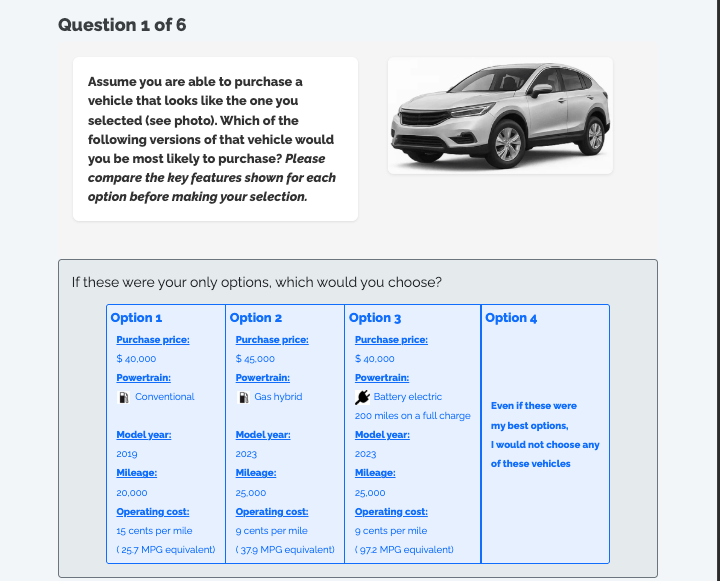
\includegraphics[width=0.7\textwidth]{images/vehicle_analysis/vehicle_choice_image.png}
    \caption{Example of a vehicle choice task presented to respondents. Each task offers three used vehicle alternatives with varying attributes and a ``None of the above'' opt-out option.}
    \label{fig:vehicle_dce}
\end{figure}

In addition to the DCE, the survey gathers information on a range of supplementary topics. Prior to the choice tasks, it collects information on respondents’ current vehicle ownership (fuel type, fuel efficiency, acquisition method, purchase or lease price, and refueling or recharging frequency) and future purchasing plans (anticipated budget, payment method, and likelihood of purchasing a new or used plug-in hybrid or BEV). Following the choice tasks, the survey assesses EV knowledge through factual questions evaluating familiarity with electrified powertrains and the federal EV tax credit, and attitudes through a series of statements rated on a 5-point Likert scale covering social norms, environmental beliefs, cost perceptions, and personality traits including risk-taking and price sensitivity. The final section collects standard demographic information --- year of birth, gender, race and ethnicity, household size, income, education level, employment status, and housing type --- as well as home ownership status and average monthly electricity expenditure.

For a comprehensive description of the survey design, see the Data Collection Instrument \parencite{goreDCIConsumerValuation2025}.\footnote{The Data Collection Instrument was published prior to the start of data collection. Certain aspects of the survey design were revised following piloting. Where discrepancies exist between the instrument and the present paper, the description in this paper reflects the final implemented version.}


\subsection{Data Collection and Sample Profile}
\label{subsec:data}

The survey was administered online between December 2025 and April 2026 through two established research platforms. Respondents were compensated through the platforms upon completion. Following initial data processing, 2,113 records were retained. The geographic distribution of respondents across the continental United States is shown in Figure~\ref{fig:map_all}; each point represents a ZIP code, with marker size and color scaled to respondent count. Median survey completion time was approximately 14 minutes.

\begin{figure}[pos=H]
    \centering
    
\includegraphics[width=0.85\textwidth]{images/map_all.png}
    \caption{Geographic distribution of survey respondents across the continental United States. Each point represents one ZIP code; marker size and color scale with respondent count.}
    \label{fig:map_all}
\end{figure}

Multiple data quality screens were then applied to identify and remove low-quality responses, including failure of an embedded attention check, within-survey response inconsistencies, and uninformative or incoherent text in open-ended fields. The final analytic sample comprises 1,500 respondents.




\section{Methods}
\label{section:methods}

\subsection{Random Utility Framework}

Consumer choice is modeled within the random utility framework. Each respondent $i$ is assumed to select the alternative $j$ that maximizes their latent utility $U_{ij}$ in each choice task, where utility is a linear function of observed vehicle attributes augmented by an unobserved idiosyncratic error term assumed to follow an independent Gumbel distribution.

\subsection{Model Specification}

A multinomial logit (MNL) model estimated via maximum likelihood provides the baseline specification under the assumption of preference homogeneity across respondents. To relax this restriction --- which is inconsistent with the substantial heterogeneity in EV attitudes documented in the literature --- the primary analysis employs a mixed logit (MXL) model. In the MXL specification, each of the eight preference parameters is modeled as an independent draw from a normal mixing distribution:

\begin{equation}
\beta_{ik} \sim \mathcal{N}(\mu_k,\, \sigma_k^2)
\label{eq:mixing}
\end{equation}

\noindent where $\mu_k$ is the population mean valuation for attribute $k$ and $\sigma_k$ captures the dispersion of that valuation across respondents. A statistically significant $\hat{\sigma}_k$ constitutes evidence that preferences for attribute $k$ are genuinely heterogeneous in the population rather than uniform. The eight parameters specified as randomly distributed are the BEV powertrain indicator, HEV powertrain indicator, BEV driving range, vehicle mileage, vehicle age, operating cost, purchase price, and the alternative-specific constant for the no-choice (opt-out) option. The internal combustion engine vehicle (ICEV) serves as the reference powertrain category throughout.

\subsection{Model Estimation}

Six MXL models are estimated, stratified by self-reported adoption propensity (likely vs.\ unlikely BEV adopter) and vehicle segment (full sample, car, SUV), yielding models for all six combinations of these two dimensions. All models are estimated in R using the \texttt{logitr} package (v1.1.2) under a preference-space specification. The mixing integral is approximated using 100 Sobol quasi-random draws per respondent. To reduce sensitivity to starting values and mitigate convergence to local optima, each model is initialized from 20 independent random starting points; the run achieving the globally lowest log-likelihood is retained. Convergence is verified via the relative and absolute function tolerance criterion (Exit Status 3) in all six models.

\subsection{Willingness-to-Pay Estimation}

Willingness to pay for attribute $k$ is derived as the negative ratio of the mean attribute coefficient to the mean price coefficient:

\begin{equation}
\widehat{\text{WTP}}_k = -\frac{\hat{\mu}_k}{\hat{\mu}_{\text{price}}}
\label{eq:wtp}
\end{equation}

\noindent This quantity represents the dollar amount the average respondent would pay --- or require as a compensating discount --- for a one-unit change in attribute $k$, holding utility constant. Uncertainty bounds on WTP estimates are computed by drawing 10{,}000 samples from the estimated joint distribution of $(\hat{\mu}_k,\, \hat{\mu}_{\text{price}})$ and reporting the resulting 95\% simulation interval.

\section{Results and Discussion}

\subsection{Model Selection}
\label{subsec:model_selection}

The MXL specification is preferred over the MNL for two related reasons. First, the estimated standard deviation parameters $\hat{\sigma}_k$ are statistically significant for virtually all attributes across all six models, confirming genuine preference heterogeneity and the violation of the MNL's representative-consumer assumption. Second, the MXL accommodates flexible substitution patterns across the qualitatively distinct powertrain alternatives. McFadden $R^2$ values range from 0.164 to 0.229 across the six specifications, within the range conventionally interpreted as indicative of good model fit for discrete choice models. The model for car-segment unlikely adopters achieves the highest fit (0.229), while the SUV-segment likely-adopter model yields the lowest (0.164), reflecting greater idiosyncratic preference variation among SUV buyers who are otherwise positively oriented toward BEVs.

\subsection{WTP for Used BEVs by Adoption Preference, Vehicle Type, and Driving Range}
\label{subsec:wtp_range}

Figure~\ref{fig:wtp_adopter_age2} presents WTP estimates at a fixed vehicle age of two years, disaggregated by adoption preference (likely vs.\ unlikely BEV adopter), vehicle type (car vs.\ SUV), and driving range (100, 200, and 300 miles). The reference value of \$0 marks the ICE-parity threshold: WTP above this line indicates a consumer-perceived premium for the used BEV relative to an equivalent ICE vehicle; WTP below it indicates the magnitude of discount required to reach purchase indifference.

\begin{figure}[pos=H]
    \centering
    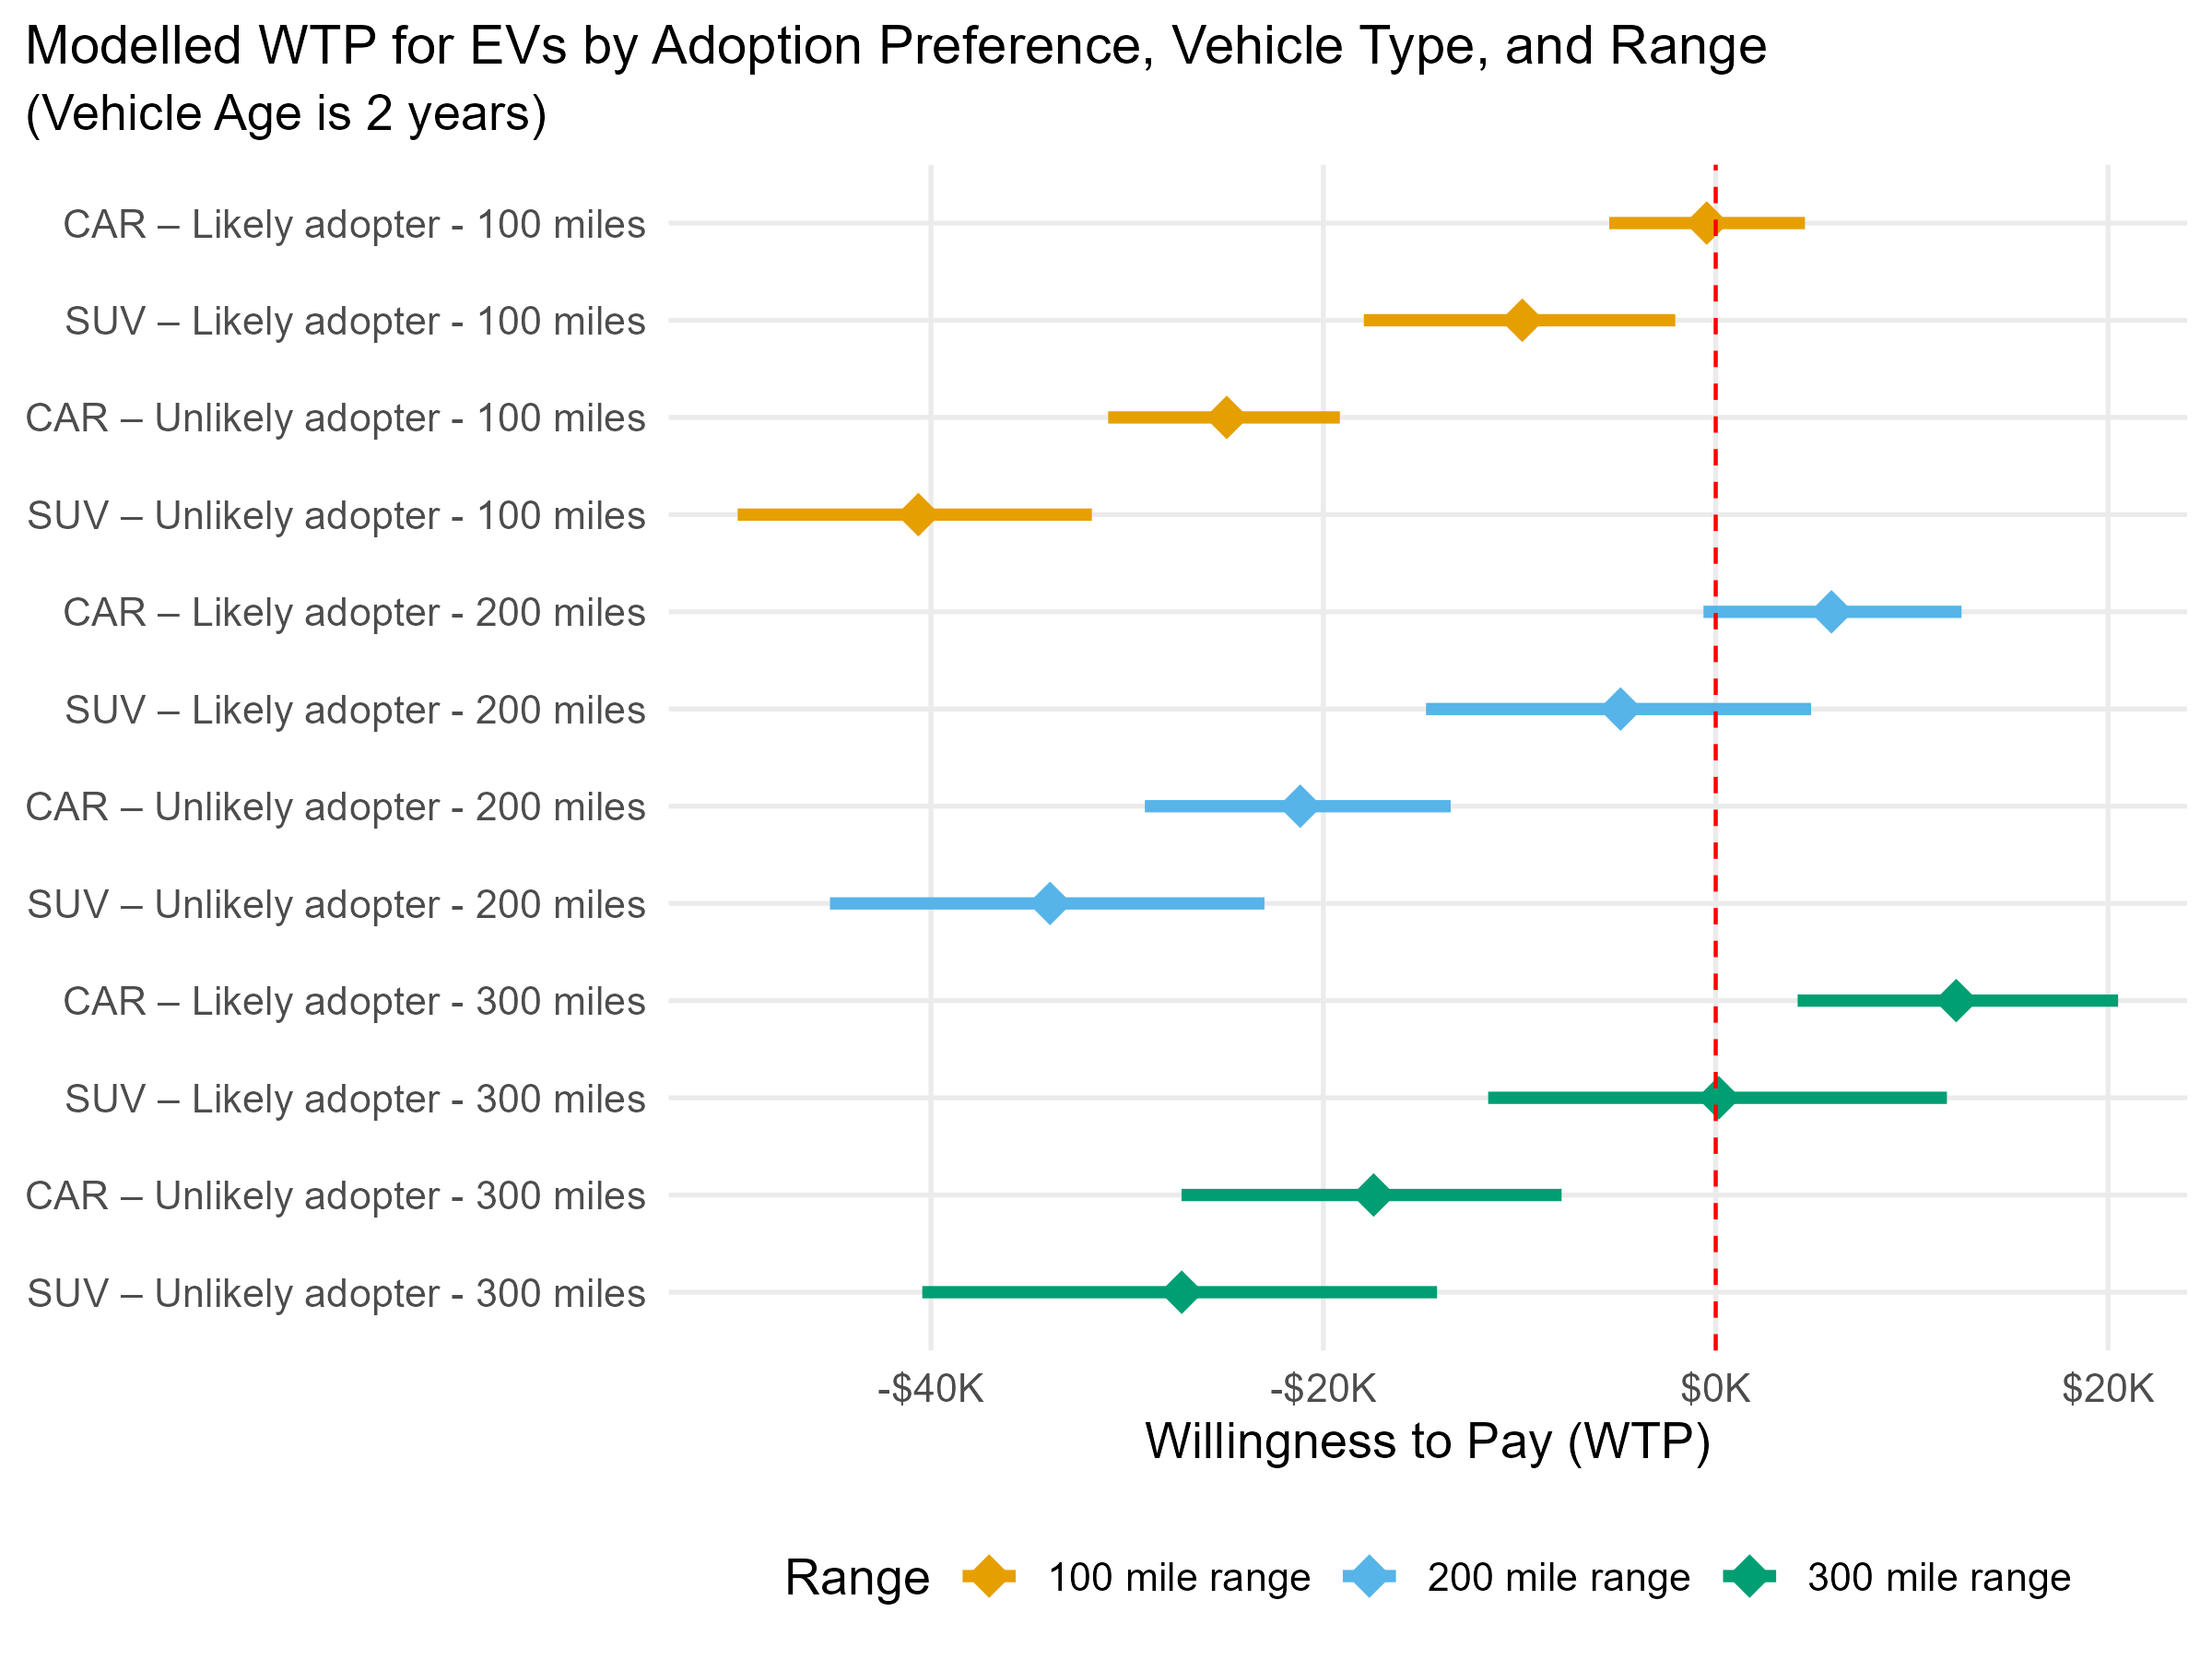
\includegraphics[width=0.85\textwidth]{images/dumbbell_plots/dumbbell_wtp_age_fixed_age_2_adopters.png}
    \caption{Modelled WTP for used BEVs by adoption preference, vehicle type, and driving range (vehicle age fixed at 2 years). Points show point estimates; horizontal bars show 95\% simulation confidence intervals.}
    \label{fig:wtp_adopter_age2}
\end{figure}

Likely adopters consistently exhibit higher WTP than unlikely adopters across all attribute combinations, and the gap is substantial. Among likely car adopters at 300-mile range, WTP is the only estimate that crosses into positive territory --- approximately \$10{,}000 to \$15{,}000 above parity --- indicating a willingness to pay a premium for a used BEV over an equivalent ICE vehicle at this combination of attributes. All other segments require a discount to induce purchase, and the required discount increases sharply with declining range and greater adoption reluctance. Unlikely adopters at 100-mile range require discounts of \$35{,}000 to \$40{,}000 relative to an ICE alternative. SUVs carry consistently lower WTP than cars within each adoption group at equivalent range levels, a vehicle-type penalty that persists across the full range of estimates.

\subsection{WTP by Adoption Preference, Vehicle Type, and Vehicle Age}
\label{subsec:wtp_age}

Figure~\ref{fig:wtp_adopter_range300} holds driving range constant at 300 miles and examines how WTP evolves across vehicle age cohorts (2, 5, and 8 years), disaggregated by adoption preference and vehicle type.

\begin{figure}[pos=H]
    \centering
    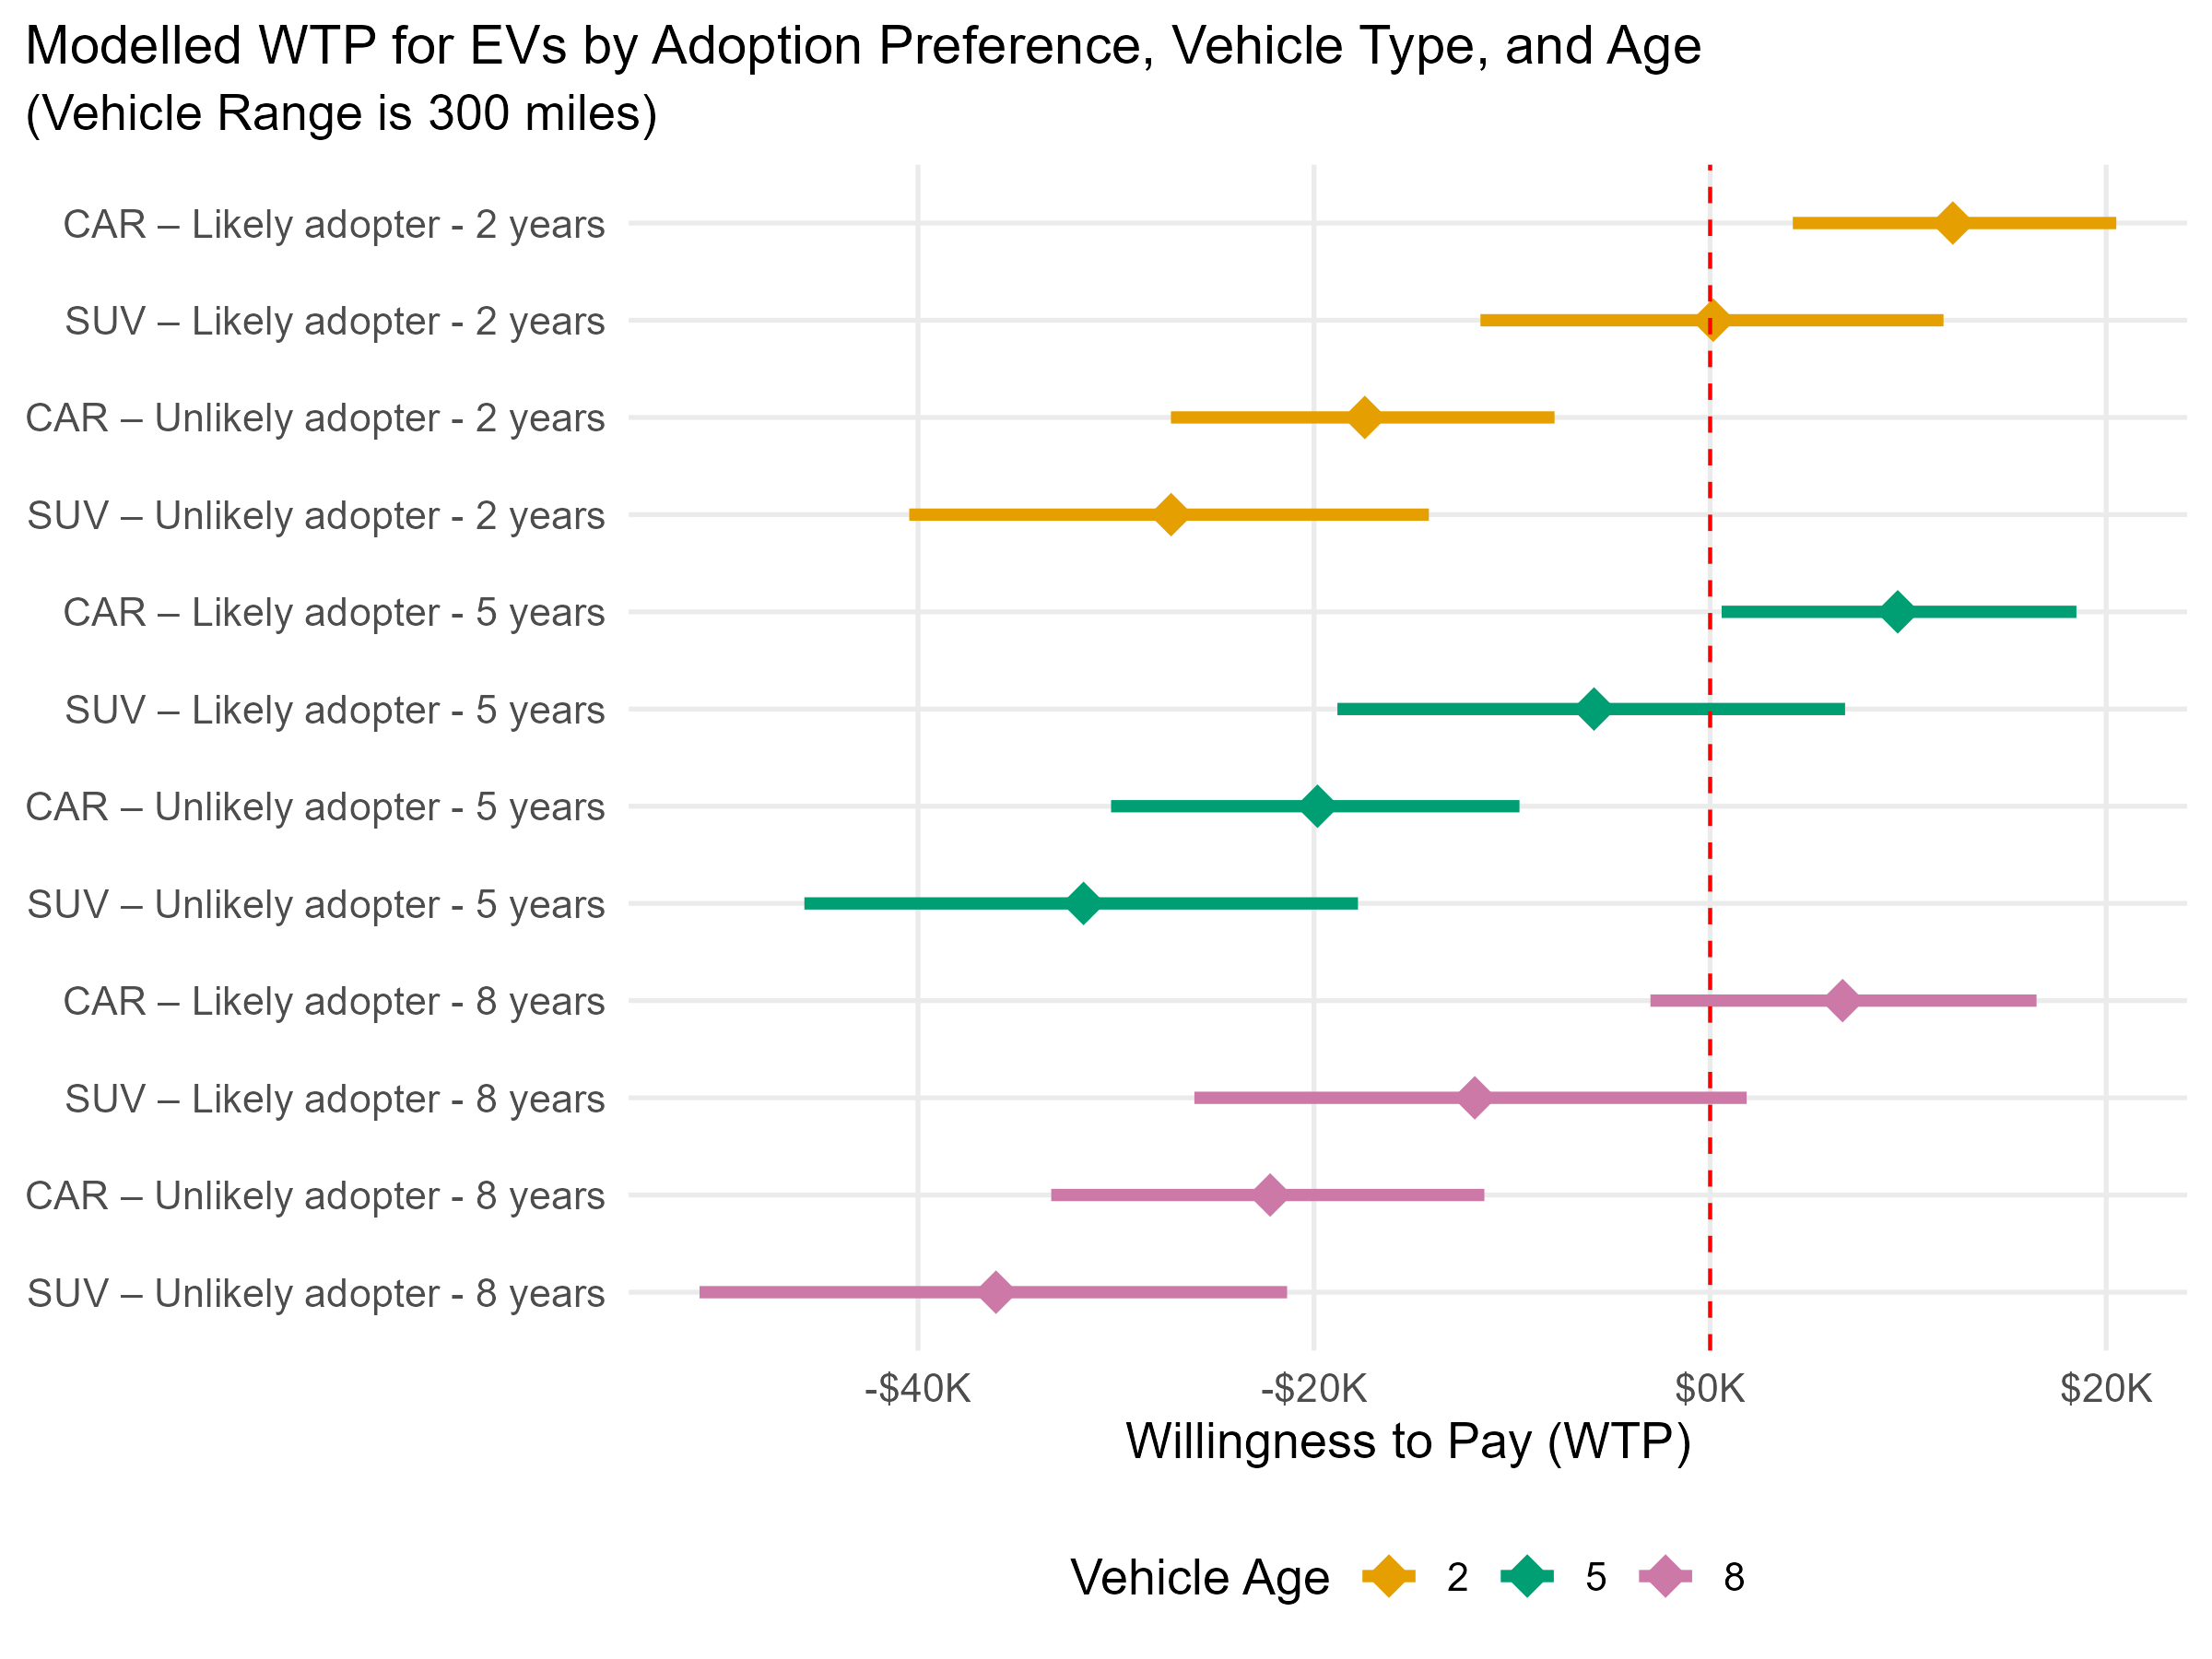
\includegraphics[width=0.85\textwidth]{images/dumbbell_plots/dumbbell_wtp_age_fixed_range_300_adopters.png}
    \caption{Modelled WTP for used BEVs by adoption preference, vehicle type, and vehicle age (driving range fixed at 300 miles). Points show point estimates; horizontal bars show 95\% simulation confidence intervals.}
    \label{fig:wtp_adopter_range300}
\end{figure}

Vehicle age exerts a large, negative, and monotonic effect on WTP. Each successive age cohort shifts estimated WTP further below the parity threshold, and the gradient exceeds what standard ICE depreciation schedules would predict for the same age interval --- an excess discount most plausibly reflecting consumer uncertainty about battery state-of-health in older vehicles rather than mechanical wear per se. The age penalty is most severe among unlikely adopters: 8-year-old SUVs in this group require discounts approaching \$40{,}000. Likely adopters are more resilient to vehicle aging --- their WTP for cars remains at or near \$0 at five years --- but shifts meaningfully downward by eight years. The joint variation in adoption preference and vehicle age produces the widest spread of WTP estimates across all model outputs, establishing these two dimensions as the primary value-determining axes in the used BEV market.

\subsection{WTP by Budget Tier, Vehicle Type, and Vehicle Age}
\label{subsec:wtp_budget}

Figure~\ref{fig:wtp_budget_range300} focuses on high-budget consumers at 300-mile range and presents WTP estimates across vehicle types and age cohorts.

\begin{figure}[pos=H]
    \centering
    
\includegraphics[width=0.85\textwidth]{images/dumbbell_plots/dumbbell_wtp_age_fixed_range_300_budgets.png}
    \caption{Modelled WTP for used BEVs by vehicle type and vehicle age --- high-budget consumers, driving range fixed at 300 miles. Points show point estimates; horizontal bars show 95\% simulation confidence intervals.}
    \label{fig:wtp_budget_range300}
\end{figure}

High-budget car buyers at two years of age represent the segment most proximate to price parity: the point estimate approaches \$0 with a confidence interval that extends into positive territory, indicating that near-parity pricing is a feasible market outcome for this specific attribute combination. The age penalty operates with similar force in this segment, with a WTP differential of approximately \$15{,}000 to \$20{,}000 between 2- and 8-year-old vehicles. SUVs lag behind cars at every age level within the high-budget group, and confidence intervals are notably wider throughout this segment, reflecting the greater estimated preference heterogeneity among SUV buyers.

\subsection{Summary of Attribute Effects on WTP}
\label{subsec:summary}

Table~\ref{table:wtp_summary} summarizes the direction and relative magnitude of each attribute's effect on WTP for used BEVs, which is consistent in sign across all model specifications.

\begin{table}[pos=H]
\caption{Direction and relative magnitude of attribute effects on WTP for used BEVs, consistent across all model specifications.}
\label{table:wtp_summary}
\centering
{\renewcommand{\arraystretch}{1.3}
\begin{tabular}{lll}
\toprule
\textbf{Attribute} & \textbf{Direction of effect on WTP} & \textbf{Relative magnitude} \\
\midrule
Driving range (100 $\to$ 300 miles)          & Positive         & Large    \\
Vehicle age (2 $\to$ 8 years)                & Negative         & Large    \\
Adoption preference (unlikely $\to$ likely)  & Positive         & Large    \\
Budget tier (low $\to$ high)                 & Positive         & Moderate \\
Vehicle type (SUV vs.\ car)                  & Negative for SUV & Moderate \\
\bottomrule
\end{tabular}}
\end{table}

Driving range, vehicle age, and adoption preference are the dominant value determinants, each producing WTP effects that substantially exceed those of budget tier and vehicle type. The only segment for which WTP reaches or exceeds the ICE-parity threshold is likely BEV adopters selecting 300-mile-range cars at two years of age. For all other attribute combinations, used BEVs must be offered at a discount, with the required discount scaling predictably with increasing vehicle age, declining range, and greater adoption reluctance.

\subsection{Mixed Logit Estimates: Preference Heterogeneity by Adoption Group}
\label{subsec:mxl_results}

Tables~\ref{table:mxl_likely} and~\ref{table:mxl_unlikely} report the full MXL parameter estimates for all six models, grouped by adoption propensity. For each attribute, the population mean coefficient ($\hat{\mu}$) and the absolute value of the estimated standard deviation of the mixing distribution ($|\hat{\sigma}|$) are presented in paired rows. A statistically significant $|\hat{\sigma}|$ indicates genuine preference heterogeneity for that attribute within the subgroup. Model fit statistics are reported at the base of each table.

\begin{table}[pos=H]
\caption{Mixed logit parameter estimates --- Likely BEV adopters. $\hat{\mu}$: population mean coefficient. $|\hat{\sigma}|$: absolute value of the estimated standard deviation of the mixing distribution; significance indicates genuine preference heterogeneity. ICEV is the reference powertrain category. Estimation: \texttt{logitr} v1.1.2 (R), 100 Sobol draws, 20 multistart runs.}
\label{table:mxl_likely}
\begin{adjustbox}{width=\textwidth, center}
{\renewcommand{\arraystretch}{1.25}
\begin{tabular}{lrrr}
\toprule
\textbf{Parameter} & \textbf{Full sample (M1)} & \textbf{Car (M3)} & \textbf{SUV (M5)} \\
\midrule
\multicolumn{4}{l}{\textit{Powertrain (ref.: ICEV)}} \\[2pt]
\quad BEV, $\hat{\mu}$               & $-0.491^{*}$    & $-1.005^{***}$  & $-1.882^{***}$ \\
\quad\quad $|\hat{\sigma}|$          & $2.159^{***}$   & $2.645^{***}$   & $3.188^{***}$  \\[3pt]
\quad HEV, $\hat{\mu}$               & $\phantom{-}0.947^{***}$  & $\phantom{-}0.914^{***}$ & $\phantom{-}0.892^{***}$ \\
\quad\quad $|\hat{\sigma}|$          & $1.728^{***}$   & $1.200^{**}$    & $1.884^{***}$  \\[3pt]
\multicolumn{4}{l}{\textit{BEV-specific attribute}} \\[2pt]
\quad BEV driving range, $\hat{\mu}$ & $\phantom{-}0.429^{***}$  & $\phantom{-}1.061^{***}$ & $\phantom{-}0.653^{***}$ \\
\quad\quad $|\hat{\sigma}|$          & $1.141^{***}$   & $0.781^{*}$     & $0.723^{**}$   \\[3pt]
\multicolumn{4}{l}{\textit{Vehicle attributes}} \\[2pt]
\quad Mileage, $\hat{\mu}$           & $-0.491^{***}$  & $-0.405^{***}$  & $-0.543^{***}$ \\
\quad\quad $|\hat{\sigma}|$          & $0.384^{**}$    & $0.093$         & $0.498^{*}$    \\[3pt]
\quad Vehicle age, $\hat{\mu}$       & $-0.233^{***}$  & $-0.154^{***}$  & $-0.283^{***}$ \\
\quad\quad $|\hat{\sigma}|$          & $0.261^{***}$   & $0.256^{**}$    & $0.217^{.}$    \\[3pt]
\multicolumn{4}{l}{\textit{Cost attributes}} \\[2pt]
\quad Operating cost, $\hat{\mu}$    & $-1.929^{***}$  & $-2.055^{***}$  & $-1.894^{***}$ \\
\quad\quad $|\hat{\sigma}|$          & $2.178^{***}$   & $2.488^{***}$   & $2.375^{***}$  \\[3pt]
\quad Purchase price, $\hat{\mu}$    & $-1.663^{***}$  & $-1.792^{***}$  & $-1.493^{***}$ \\[3pt]
\multicolumn{4}{l}{\textit{No-choice (opt-out) constant}} \\[2pt]
\quad $\hat{\mu}$                    & $-16.500^{***}$ & $-20.546^{***}$ & $-14.497^{***}$\\
\quad\quad $|\hat{\sigma}|$          & $7.211^{***}$   & $10.728^{***}$  & $4.264^{***}$  \\
\midrule
\multicolumn{4}{l}{\textit{Model fit}} \\[2pt]
\quad Observations                   & 5,028           & 2,538           & 2,490          \\
\quad Log-likelihood                 & $-5{,}698.14$   & $-2{,}766.11$   & $-2{,}884.44$  \\
\quad McFadden $R^{2}$               & 0.183           & 0.214           & 0.164          \\
\bottomrule
\multicolumn{4}{p{\dimexpr\linewidth-2\tabcolsep\relax}}{\footnotesize
  Significance: $^{***}p<0.001$; $^{**}p<0.01$; $^{*}p<0.05$; $^{.}p<0.10$; blank = not significant.} \\
\end{tabular}}
\end{adjustbox}
\end{table}

As shown in Table~\ref{table:mxl_likely}, the six MXL models establish that the aggregate WTP patterns in Figures~\ref{fig:wtp_adopter_age2}--\ref{fig:wtp_budget_range300} reflect qualitatively distinct preference structures across adoption groups, with substantial within-group heterogeneity characterizing both segments. Among likely BEV adopters, mean BEV powertrain coefficients are negative across all three vehicle-segment specifications (full sample: $\hat{\mu} = -0.49$; car: $\hat{\mu} = -1.01$; SUV: $\hat{\mu} = -1.88$), yet are accompanied in each case by large and statistically significant standard deviations ($|\hat{\sigma}| = 2.2$--$3.2$, $p < 0.001$ throughout). The apparent contradiction between negative mean BEV utility and self-reported adoption likelihood is resolved by the mixing distribution: simulation-based draws confirm that the interquartile range for BEV utility straddles zero within each subgroup, indicating genuine within-group polarization. HEV powertrains are, by contrast, unambiguously preferred over the ICEV baseline among likely adopters ($\hat{\mu} = 0.89$--$0.95$, $p < 0.001$), suggesting that hybrid electrification represents the more broadly accepted form of powertrain transition within this group. Driving range is the dominant positive attribute among likely car adopters ($\hat{\mu} = 1.061$, $p < 0.001$) --- approximately 2.5 times its magnitude in the full likely-adopter sample --- identifying range as the primary attribute lever for this subgroup.

\begin{table}[pos=H]
\caption{Mixed logit parameter estimates --- Unlikely BEV adopters. $\hat{\mu}$: population mean coefficient. $|\hat{\sigma}|$: absolute value of the estimated standard deviation of the mixing distribution; significance indicates genuine preference heterogeneity. ICEV is the reference powertrain category. Estimation: \texttt{logitr} v1.1.2 (R), 100 Sobol draws, 20 multistart runs.}
\label{table:mxl_unlikely}
\begin{adjustbox}{width=\textwidth, center}
{\renewcommand{\arraystretch}{1.25}
\begin{tabular}{lrrr}
\toprule
\textbf{Parameter} & \textbf{Full sample (M2)} & \textbf{Car (M4)} & \textbf{SUV (M6)} \\
\midrule
\multicolumn{4}{l}{\textit{Powertrain (ref.: ICEV)}} \\[2pt]
\quad BEV, $\hat{\mu}$               & $-7.776^{***}$  & $-9.273^{***}$  & $-8.347^{***}$ \\
\quad\quad $|\hat{\sigma}|$          & $5.207^{***}$   & $6.510^{***}$   & $5.161^{***}$  \\[3pt]
\quad HEV, $\hat{\mu}$               & $-0.734^{***}$  & $-0.758^{***}$  & $-0.617^{***}$ \\
\quad\quad $|\hat{\sigma}|$          & $3.072^{***}$   & $3.432^{***}$   & $2.671^{***}$  \\[3pt]
\multicolumn{4}{l}{\textit{BEV-specific attribute}} \\[2pt]
\quad BEV driving range, $\hat{\mu}$ & $\phantom{-}0.488^{*}$   & $\phantom{-}0.420$        & $\phantom{-}0.790^{***}$ \\
\quad\quad $|\hat{\sigma}|$          & $0.843^{**}$    & $2.194^{***}$   & $0.722^{*}$    \\[3pt]
\multicolumn{4}{l}{\textit{Vehicle attributes}} \\[2pt]
\quad Mileage, $\hat{\mu}$           & $-0.523^{***}$  & $-0.559^{***}$  & $-0.508^{***}$ \\
\quad\quad $|\hat{\sigma}|$          & $0.455^{***}$   & $0.772^{***}$   & $0.103$        \\[3pt]
\quad Vehicle age, $\hat{\mu}$       & $-0.200^{***}$  & $-0.185^{***}$  & $-0.218^{***}$ \\
\quad\quad $|\hat{\sigma}|$          & $0.165^{**}$    & $0.083$         & $0.105$        \\[3pt]
\multicolumn{4}{l}{\textit{Cost attributes}} \\[2pt]
\quad Operating cost, $\hat{\mu}$    & $-1.788^{***}$  & $-2.026^{***}$  & $-1.718^{***}$ \\
\quad\quad $|\hat{\sigma}|$          & $1.711^{***}$   & $1.953^{***}$   & $1.868^{***}$  \\[3pt]
\quad Purchase price, $\hat{\mu}$    & $-2.145^{***}$  & $-2.912^{***}$  & $-1.743^{***}$ \\[3pt]
\multicolumn{4}{l}{\textit{No-choice (opt-out) constant}} \\[2pt]
\quad $\hat{\mu}$                    & $-16.470^{***}$ & $-18.493^{***}$ & $-14.204^{***}$\\
\quad\quad $|\hat{\sigma}|$          & $6.046^{***}$   & $6.198^{***}$   & $4.180^{***}$  \\
\midrule
\multicolumn{4}{l}{\textit{Model fit}} \\[2pt]
\quad Observations                   & 6,714           & 3,222           & 3,492          \\
\quad Log-likelihood                 & $-7{,}345.44$   & $-3{,}442.62$   & $-3{,}866.73$  \\
\quad McFadden $R^{2}$               & 0.211           & 0.229           & 0.201          \\
\bottomrule
\multicolumn{4}{p{\dimexpr\linewidth-2\tabcolsep\relax}}{\footnotesize
  Significance: $^{***}p<0.001$; $^{**}p<0.01$; $^{*}p<0.05$; $^{.}p<0.10$; blank = not significant. BEV driving range (M4): $\hat{\mu} = 0.420$, $p = 0.272$ (not significant).} \\
\end{tabular}}
\end{adjustbox}
\end{table}

Among unlikely BEV adopters (Table~\ref{table:mxl_unlikely}), the preference structure is categorically different. Mean BEV utility coefficients are large and negative across all three models (full sample: $\hat{\mu} = -7.78$; car: $\hat{\mu} = -9.27$; SUV: $\hat{\mu} = -8.35$; all $p < 0.001$), with simulation-based draws confirming near-universal aversion in the car segment: at least 75\% of the simulated population holds strongly negative BEV utility, with effectively no probability mass above zero. HEV powertrains are also negatively valued ($\hat{\mu} = -0.62$ to $-0.76$, $p < 0.001$), establishing that the resistance extends to electrification broadly rather than to BEVs specifically. Price sensitivity among unlikely adopters substantially exceeds that of likely adopters: the price coefficient for car-segment unlikely adopters ($\hat{\mu} = -2.912$) is 63\% larger in magnitude than for the corresponding likely-adopter group ($\hat{\mu} = -1.792$), and the full-sample differential is approximately 29\%. Driving range is a statistically significant predictor of vehicle choice in five of the six models; the single exception is the car-segment unlikely-adopter model ($\hat{\mu} = 0.420$, $p = 0.272$), indicating that range improvements alone would not induce BEV consideration among this segment's car buyers. Despite the pervasive aversion, large standard deviations on both BEV and HEV coefficients ($|\hat{\sigma}_{\text{BEV}}| = 5.2$--$6.5$; $|\hat{\sigma}_{\text{HEV}}| = 2.7$--$3.4$, all $p < 0.01$) confirm that a non-trivial minority within the unlikely-adopter population holds more favorable powertrain views --- particularly in the SUV segment, where mean HEV aversion is weakest ($\hat{\mu} = -0.617$) and where hybrid vehicles may represent a more tractable intermediate adoption pathway.

\section{Conclusion}
\label{section:conclusion}

This study provides quantitative estimates of consumer willingness to pay for used battery electric vehicles in the United States, disaggregated by adoption propensity, vehicle type, driving range, vehicle age, and budget tier. A discrete choice experiment administered to 1{,}500 prospective used-vehicle buyers yielded six mixed logit models that recover preference parameters and characterize heterogeneity across adoption and vehicle segments.

Three findings carry direct implications for used BEV market development. First, the used BEV market has not reached price parity with conventional vehicles for the majority of prospective buyers: only likely BEV adopters selecting 300-mile-range cars at two years of age demonstrate WTP at or near the ICE-equivalent price, while all other segment combinations require discounts ranging from modest to over \$35{,}000. Second, vehicle age is a first-order negative driver of WTP across all segments, with an estimated WTP differential of \$15{,}000 to \$20{,}000 between 2-year-old and 8-year-old vehicles within a given segment. This excess discount relative to standard ICE depreciation most plausibly reflects consumer uncertainty about battery state-of-health, suggesting that interventions improving SOH transparency --- standardized health disclosures, third-party certification, or extended manufacturer warranties in the secondary market --- could recover a portion of this penalty without requiring changes to the vehicle itself. Third, driving range is the primary positive attribute for likely BEV adopters, particularly in the car segment, yet range has no statistically significant effect among car-segment unlikely adopters, establishing that range improvements alone are insufficient to expand adoption into the most resistant consumer group.

These findings point to a segmented market in which no single pricing or policy instrument is uniformly effective. For likely adopters --- the population proximate to the purchase threshold --- communication strategies emphasizing driving range sufficiency and per-mile operating cost advantages are the most efficient levers for conversion, given this group's high purchase engagement and elevated operating cost sensitivity. For unlikely adopters, whose BEV aversion is near-universal and price sensitivity is 29--63\% higher than among likely adopters depending on the segment, the federal used EV tax credit (currently capped at \$4{,}000) falls well short of the discounts required to reach purchase indifference. The most tractable near-term intervention for this population is the promotion of hybrid electric vehicles, particularly in the SUV segment, where within-group HEV heterogeneity indicates a non-trivial receptive minority. State-level programs designed with segment awareness --- concentrating on high-budget car buyers at low vehicle age, where the market is already proximate to parity --- would achieve better marginal additionality than uniform subsidies applied irrespective of vehicle age, range, or buyer propensity.

Several limitations bound the scope of these findings. The analysis rests on stated rather than revealed preferences; hypothetical bias may affect WTP magnitudes, though its direction in this context is uncertain. The sample was drawn from online research panels and may overrepresent information-engaged consumers. The MXL specification assumes continuous normal mixing distributions, which may inadequately represent discrete preference clusters; a latent class extension would test this directly. Battery state-of-health was not varied in the vehicle powertrain DCE analyzed here and is addressed in a companion battery DCE component of the broader study. Integrating findings from both instruments and cross-validating against revealed transaction prices from dealer records would substantially strengthen the empirical basis for the policy inferences drawn above.

\printcredits


\printbibliography


\end{document}